% ------------------------------------------------------------------
\renewcommand{\thisunit}{MATH327 Unit 6}
\renewcommand{\moddate}{Last modified 12 Feb.~2022}
\setcounter{section}{6}
\setcounter{subsection}{0}
\phantomsection
\addcontentsline{toc}{section}{Unit 6: Grand-canonical ensemble}
\section*{Unit 6: Grand-canonical ensemble}
\subsection{The particle reservoir and chemical potential}
This week we define and develop the third and final statistical ensemble to be studied in this module, which is known as the grand-canonical ensemble.
Our approach will follow the pattern set by our previous development of the canonical ensemble.
Recall that statistical ensembles are probability spaces describing the micro-states that a system can adopt as it evolves in time, subject to certain constraints.
We began in week 2 with the micro-canonical ensemble, in which these constraints were conservation of the internal energy $E$ and particle number $N$.
We then introduced the canonical ensemble in week 3 by allowing the system's internal energy to fluctuate, while keeping its temperature $T$ fixed through thermal contact with a large external thermal reservoir.

The next step is to allow \textit{both} the system's energy and its particle number to fluctuate.
Just as we saw for the canonical ensemble in week 3, these fluctuations occur through contact between the system and a large external reservoir.
This is now a \textbf{particle reservoir}, with which the system can exchange both energy and particles.

In the same way that energy exchange leads to a fixed temperature, we expect there to be some quantity that will be fixed due to particle exchange.
Recall that we initially defined the temperature in the context of the micro-canonical ensemble in thermodynamic equilibrium (\eq{eq:temperature}), as the dependence of the entropy on the internal energy for a fixed number of degrees of freedom:
\begin{equation*}
  \frac{1}{T} = \left. \pderiv{S}{E}\right|_N.
\end{equation*}
The quantity we are now interested in comes from the complementary analysis interchanging the roles of $E$ and $N$.

\begin{shaded}
  In thermodynamic equilibrium, the \textbf{chemical potential} in the micro-canonical ensemble is defined by
  \begin{equation}
    \label{eq:chem_pot}
    \mu = -T \left. \pderiv{S}{N}\right|_E.
  \end{equation}
\end{shaded}

This definition is not terribly intuitive, nor is the chemical potential a familiar concept from everyday experiences.
To gain some insight into the chemical potential, we can note (from either \eq{eq:temperature} or \eq{eq:first_law}) that $\mu$ has dimensions of energy.
We can also expect the partial derivative $\pderiv{S}{N}$ to be positive in general, since systems with more degrees of freedom generically have more entropy, reflecting the greater amount of information they can contain.
This can be checked explicitly for the spin system (\eq{eq:dist_entropy}) and ideal gas (\eq{eq:ideal_entropy}) we previously analyzed.
The choice of sign in \eq{eq:chem_pot} therefore means that we should expect the chemical potential to be negative, in `natural' systems with positive temperatures.

The motivation for this negative sign comes from considering a net flow of particles between two systems $\Om_A$ and $\Om_B$ with the same temperature $T$ but different
\begin{equation*}
  \left(\pderiv{S}{N}\right)_A > \left(\pderiv{S}{N}\right)_B \qquad \Lra \qquad \mu_A < \mu_B.
\end{equation*}
Due to the negative sign in \eq{eq:chem_pot}, the system with the larger partial derivative has the smaller (more-negative) chemical potential.
According to the second law of thermodynamics, particles will flow from $\Om_B$ to $\Om_A$, because
\begin{equation*}
  \De S_A = \left(\pderiv{S}{N}\right)_A \De N > \left(\pderiv{S}{N}\right)_B \De N = \De S_B,
\end{equation*}
meaning that more entropy is gained by adding particles to system $\Om_A$ than is lost by removing particles from system $\Om_B$.
This ensures that the process increases the total entropy of the universe, $\De S = \De S_A - \De S_B > 0$.
In other words, we expect particles to flow \textit{from} systems with larger chemical potentials \textit{to} systems with smaller chemical potential.
This provides a useful similarity to heat flowing from hotter systems with larger temperatures to colder systems with smaller temperatures, allowing us to borrow our intuition from temperature to apply to the less-familiar chemical potential.\footnote{Of course, the mathematics would work just as well with the opposite sign convention---in that case we would just need to develop the opposite intuition for chemical potential vs.\ temperature.}
Like the temperature, the chemical potential is an intensive quantity.

\begin{shaded}
  We are now able to define the \textbf{grand-canonical ensemble} to be a statistical ensemble characterized by its fixed temperature $T$ and fixed chemical potential $\mu$, with the temperature and chemical potential held fixed through contact with a particle reservoir.
\end{shaded}
% ------------------------------------------------------------------



% ------------------------------------------------------------------
\subsection{\label{sec:Zg}The grand-canonical partition function}
We now place the grand-canonical ensemble on a more concrete mathematical foundation, following the same path as we did when developing the canonical ensemble.
That is, we introduce a well-motivated ansatz for the form of the particle reservoir $\Om_{\text{res}}$, then show that this specific form of $\Om_{\text{res}}$ is ultimately irrelevant.
This will allow us to work directly with the system of interest, $\Om$, independent of the details of the particle reservoir that fixes its temperature and chemical potential.

As before, our ansatz is to take $\Om_{\text{tot}} = \Om_{\text{res}} \otimes \Om$ to consist of many ($R \gg 1$) identical replicas of the system \Om that we're interested in.
All of these replicas are in thermodynamic equilibrium, and can exchange both energy and particles with each other.
The overall system $\Om_{\text{tot}}$ is governed by the micro-canonical ensemble, with conserved total energy \Etot and conserved total particle number $\Ntot$.
An extremely small example of this setup is illustrated by the figure below, where the system of interest is an ideal gas in a volume $V$.
This week we will consider only indistinguishable particles, so that we don't need to keep track of which particular particles are exchanged between the replicas, only the overall number.

\begin{center}
  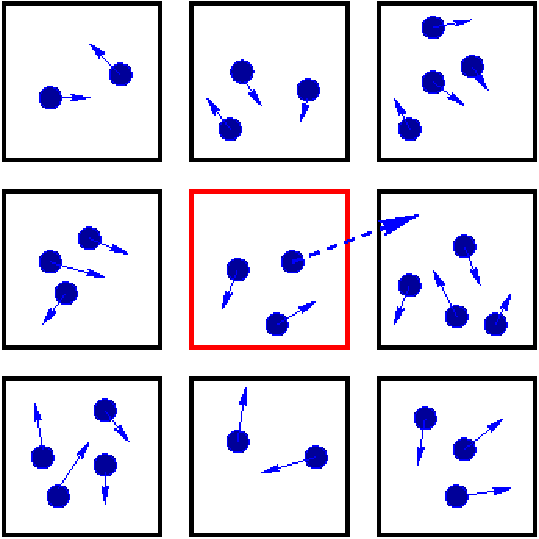
\includegraphics[width=0.7\textwidth]{figs/unit06_reservoir.pdf}
\end{center}

Although we draw a box around each replica (and colour one red to pick out the system \Om we will consider), these boxes are now merely mental constructions, and don't interfere with particles moving from one replica to another.
For example, we could take our system to be a cubic centimetre of air in a room, with the rest of the room forming its reservoir.
As in \secref{sec:replicas}, we assume that this system $\Om = \left\{\om_1, \om_2, \cdots, \om_M\right\}$ has a finite number of $M$ possible micro-states, where now different micro-states may involve different numbers of particles.

This again allows us to analyze the overall system of $R$ replicas in terms of occupation numbers $n_i$ and the corresponding occupation probabilities $p_i$.
Recall that $n_i$ is the number of replicas that adopt the micro-state $\om_i \in \Om$ in any given micro-state of the overall system $\Om_{\text{tot}}$, so that $\sum_i n_i = R$.
Similarly, $p_i = n_i / R$ is the probability that a randomly chosen replica will be in micro-state $\om_i$, with $\sum_i p_i = 1$ as usual.
In terms of $n_i$ and $p_i$, the total number of micro-states of $\Om_{\text{tot}}$, and the corresponding entropy, are the same as we derived in \secref{sec:canon_part},
\begin{equation*}
  M_{\text{tot}} = \frac{R!}{n_1! \; n_2! \; \cdots \; n_M!} \qquad \lra \qquad S(\Etot, \Ntot) = -R \sum_{i = 1}^M p_i \log p_i,
\end{equation*}
assuming $R \gg 1$ and $n_i \gg 1$ for all $i = 1, \cdots, M$.
In this expression, the dependence on both \Etot and \Ntot now enters through the occupation probabilities $p_i$, since the micro-states $\om_i$ may involve different numbers of particles in addition to different energies.

Continuing as before, we want to determine the (intensive) temperature and chemical potential of $\Om_{\text{tot}}$ through Eqs.~\ref{eq:temperature} and \ref{eq:chem_pot}, which requires expressing $S(\Etot, \Ntot)$ directly in terms of \Etot and $\Ntot$.
We again do this by maximizing the entropy subject to the constraints on the conserved quantities of the micro-canonical overall system $\Om_{\text{tot}}$.
Labelling the energy and particle number of each replica $E_r$ and $N_r$, respectively, as in \eq{eq:canon_Etot} we can again rearrange sums over replicas into sums over the micro-states of $\Om$:
\begin{align}
  1 & = \sum_{i = 1}^M p_i & \Etot = \sum_{r = 1}^R E_r = \sum_{i = 1}^M n_i E_i & = R \sum_{i = 1}^M p_i E_i \cr
    &                      & \Ntot = \sum_{r = 1}^R N_r = \sum_{i = 1}^M n_i N_i & = R \sum_{i = 1}^M p_i N_i, \label{eq:grand_constraint}
\end{align}
where $E_i$ and $N_i$ are the energies and particle numbers of the $M$ micro-states $\om_i \in \Om$.
The first two constraints, on the occupation probabilities and the total energy, are the same as we had in \secref{sec:canon_part}.
The third constraint, on the total particle number, is the new ingredient for us to incorporate.

Writing everything in terms of occupation probabilities (choosing signs and normalization factors for later convenience), we see that we need to maximize the modified entropy
\begin{align*}
  \Sbar = -R \sum_{i = 1}^M p_i \log p_i & + \al\left(\sum_{i = 1}^M p_i - 1\right) \\
                                         & - \be\left(R \sum_{i = 1}^M p_i E_i - \Etot\right) + \ga\left(R \sum_{i = 1}^M p_i N_i - \Ntot\right),
\end{align*}
with the three Lagrange multipliers $\al$, \be and $\ga$.
What is the occupation probability $p_k$ that maximizes $\Sbar$?
\begin{mdframed}
  $\displaystyle 0 = \pderiv{\Sbar}{p_k} = $ \\[140 pt] % WARNING: FORMATTING BY HAND
\end{mdframed}

You should find a probability of the form
\begin{equation}
  \label{eq:grand_Lagrange}
  p_k = \frac{1}{Z_g} e^{-\be E_k + \ga N_k},
\end{equation}
defining $Z_g = \exp\left[1 - \frac{\al}{R}\right]$ to work in terms of the parameters $\left\{Z_g, \be, \ga\right\}$.
As usual, we fix these three parameters by demanding that the three constraints above are satisfied.
Using the first constraint, what is $Z_g$ in terms of \be and $\ga$?
\begin{mdframed}
  $\displaystyle 1 = \sum_{i = 1}^M p_i = $ \\[50 pt]
\end{mdframed}

Guided by our work in \secref{sec:canon_part}, we can expect to need the partial derivatives
\begin{align}
  \frac{1}{Z_g} \pderiv{}{\be} Z_g(\be, \ga) & = \frac{1}{Z_g} \pderiv{}{\be} \sum_{i = 1}^M e^{-\be E_i + \ga N_i} = -\frac{1}{Z_g} \sum_{i = 1}^M E_i \; e^{-\be E_i + \ga N_i} = -\frac{\Etot}{R} \label{eq:grand_be_deriv} \\
  \frac{1}{Z_g} \pderiv{}{\ga} Z_g(\be, \ga) & = \frac{1}{Z_g} \pderiv{}{\ga} \sum_{i = 1}^M e^{-\be E_i + \ga N_i} = \frac{1}{Z_g} \sum_{i = 1}^M N_i \; e^{-\be E_i + \ga N_i} = \frac{\Ntot}{R} \label{eq:grand_ga_deriv},
\end{align}
where we have used $\Etot = R \sum_i p_i E_i$ and $\Ntot = R \sum_i p_i N_i$ from \eq{eq:grand_constraint}.
These partial derivatives appear when we express the entropy in terms of $\Etot$, \Ntot and the parameters
\begin{equation*}
  \left\{Z_g(\be, \ga), \quad \be(\Etot, \Ntot), \quad \ga(\Etot, \Ntot)\right\},
\end{equation*}
then take the partial derivatives that define the temperature and chemical potential.
What do you obtain upon inserting \eq{eq:grand_Lagrange} for $p_i$ into the formula for the entropy?
\begin{mdframed}
  $\displaystyle S(\Etot, \Ntot) = -R \sum_{i = 1}^M p_i \log p_i = $ \\[100 pt]
\end{mdframed}

\newpage % WARNING: FORMATTING BY HAND
Taking the derivative of the result with respect to $\Etot$, keeping \Ntot fixed, gives us the temperature (\eq{eq:temperature}):
\begin{align}
  \frac{1}{T} & = \pderiv{}{\Etot}\left[R\log Z_g + \be \Etot - \ga \Ntot\right]_{\Ntot} \cr
              & = \frac{R}{Z_g}\left(\pderiv{Z_g}{\be}\pderiv{\be}{\Etot} + \pderiv{Z_g}{\ga}\pderiv{\ga}{\Etot}\right) + \Etot\pderiv{\be}{\Etot} + \be - \Ntot\pderiv{\ga}{\Etot} \cr
              & = -\Etot\pderiv{\be}{\Etot} + \Ntot\pderiv{\ga}{\Etot} + \Etot\pderiv{\be}{\Etot} + \be - \Ntot\pderiv{\ga}{\Etot} = \be,
\end{align}
where we insert Eqs.~\ref{eq:grand_be_deriv} and \ref{eq:grand_ga_deriv} in the last line.
In the same way, the derivative with respect to $\Ntot$, keeping $\Etot$ fixed, gives us the chemical potential:
\begin{align}
  \mu & = -T \pderiv{}{\Ntot}\left[R\log Z_g + \be \Etot - \ga \Ntot\right]_{\Ntot} \cr
      & = -T\left[\frac{R}{Z_g}\left(\pderiv{Z_g}{\be}\pderiv{\be}{\Ntot} + \pderiv{Z_g}{\ga}\pderiv{\ga}{\Ntot}\right) + \Etot\pderiv{\be}{\Ntot} - \Ntot\pderiv{\ga}{\Ntot} - \ga\right] \cr
      & = -T\left[-\Etot\pderiv{\be}{\Ntot} + \Ntot\pderiv{\ga}{\Ntot} + \Etot\pderiv{\be}{\Ntot} - \Ntot\pderiv{\ga}{\Ntot} - \ga\right] = T\ga.
\end{align}

Putting everything together, we have
\begin{align}
  \be & = \frac{1}{T} &
  \ga & = \be \mu = \frac{\mu}{T}
\end{align}
and the desired result that all the details of the particle reservoir have vanished, with no remaining reference to $R$, \Etot or $\Ntot$.
The large particle reservoir is still present to fix the temperature $T$ and chemical potential $\mu$ that characterize the grand-canonical system $\Om$, but beyond that nothing about it is relevant---or even knowable in the grand-canonical approach.

Every aspect of \Om can now be specified in terms of its fixed temperature $T$ and chemical potential $\mu$, starting with the parameters $\be = 1 / T$ and $\ga = \mu / T$.
In particular, the probability---in thermodynamic equilibrium---that \Om adopts micro-state $\om_i$ with (non-conserved) internal energy $E_i$ and particle number $N_i$ is
\begin{equation}
  \label{eq:grand_prob}
  p_i = \frac{1}{Z_g} e^{-\be (E_i - \mu N_i)} = \frac{1}{Z_g} e^{-(E_i - \mu N_i) / T}.
\end{equation}

\begin{shaded}
  These probabilities depend on the \textbf{grand-canonical partition function}
  \begin{equation}
    \label{eq:grand_part_func}
    Z_g(T, \mu) = \sum_{i = 1}^M e^{-\be (E_i - \mu N_i)} = \sum_{i = 1}^M e^{-(E_i - \mu N_i) / T}.
  \end{equation}
  Analogously to the canonical partition function, this $Z_g$ is a fundamental quantity in the grand-canonical ensemble, from which many other derived quantities can be obtained.
\end{shaded}

Since the particle number $N_i$ is dimensionless, the combination $E_i - \mu N_i$ that appears in Eqs.~\ref{eq:grand_prob} and \ref{eq:grand_part_func} is consistent with our observation below \eq{eq:chem_pot} that the chemical potential $\mu$ has dimensions of energy.
% ------------------------------------------------------------------



% ------------------------------------------------------------------
\subsection{The grand-canonical potential, internal energy, entropy, and particle number}
The development of the grand-canonical ensemble we have seen so far closely resembles our earlier work setting up the canonical ensemble.
We have generalized the thermal reservoir to a particle reservoir that allows both the internal energy and particle number of the system \Om to vary, while keeping its temperature $T$ and chemical potential $\mu$ fixed.
By adapting the replica ansatz to this setup, we determined the grand-canonical partition function $Z_g$, and found it to be independent of the details of the particle reservoir.

We now continue by considering a similar set of derived quantities for the grand-canonical ensemble in thermodynamic equilibrium.
In addition to the expectation value of the internal energy introduced in \secref{sec:canon_derived}, the fluctuations of the particle number mean that we also need to consider its expectation value,
\begin{align*}
  \vev{E}\!(T, \mu) & = \sum_{i = 1}^M E_i \; p_i = \frac{1}{Z_g} \sum_{i = 1}^M E_i \; e^{-\be (E_i - \mu N_i)} \\
  \vev{N}\!(T, \mu) & = \sum_{i = 1}^M N_i \; p_i = \frac{1}{Z_g} \sum_{i = 1}^M N_i \; e^{-\be (E_i - \mu N_i)}.
\end{align*}
We can anticipate that both of these derived quantities will be related to the logarithm of the grand-canonical partition function, in analogy to the Helmholtz free energy for the canonical ensemble considered in \secref{sec:Helmholtz}.

\begin{shaded}
  This leads us to define \textbf{grand-canonical potential} of a grand-canonical ensemble to be
  \begin{equation}
    \label{eq:grand_pot}
    \Phi(T, \mu) = -T \log Z_g(T, \mu) = -\frac{\log Z_g(\be, \mu)}{\be},
  \end{equation}
  where $Z_g$ is the grand-canonical partition function of the ensemble.
  In terms of this free energy, Eqs.~\ref{eq:grand_prob} and \ref{eq:grand_part_func} are
  \begin{align*}
    Z_g & = e^{-\Phi / T} &
    p_i & = e^{(\Phi - E_i + \mu N_i) / T}.
  \end{align*}
\end{shaded}

The grand-canonical potential is sometimes called the \textit{Landau free energy}, named after \href{https://en.wikipedia.org/wiki/Lev_Landau}{Lev Landau}, to highlight its similarity with the Helmholtz free energy.
\newpage % WARNING: FORMATTING BY HAND
\noindent An aspect of this similarity is the importance of derivatives of the grand-canonical potential.
The simplest derivative to consider first is with respect to the chemical potential,
\begin{mdframed}
  $\displaystyle \pderiv{}{\mu} \Phi(\be, \mu) = $ \\[120 pt]
\end{mdframed}
The derivative with respect to the temperature is a little messier.
As in \secref{sec:Helmholtz}, it involves $\pderiv{}{T} \log Z_g$, which is again worth collecting in advance, recalling $\pderiv{}{T} = -\be^2 \pderiv{}{\be} $ from \eq{eq:beta_T}.
\begin{mdframed}
  $\displaystyle -\pderiv{}{T}\left(\frac{\Phi(T, \mu)}{T}\right) = \pderiv{}{T} \log Z_g(T, \mu) = $ \\[80 pt]
  $\displaystyle \pderiv{}{T} \Phi(T, \mu) = $ \\[80 pt]
\end{mdframed}
\newpage % WARNING: FORMATTING BY HAND
\noindent You should find
\begin{equation*}
  \pderiv{\Phi}{T} = \frac{\Phi - \vev{E} + \mu\vev{N}}{T} = -\log Z_g - \be\vev{E} + \be\mu\vev{N},
\end{equation*}
which we can connect to the entropy by inserting the probabilities $p_i$ from \eq{eq:grand_prob} into the definition of the entropy from \eq{eq:entropy}:
\begin{mdframed}
  $\displaystyle S(T, \mu) = -\sum_{i = 1}^M p_i \log p_i = $ \\[100 pt]
\end{mdframed}

\begin{shaded}
  From this work we can read off the following relations involving the grand-canonical potential $\Phi(T, \mu)$:
  \begin{align}
    \vev{N}\!(T, \mu) & = -\pderiv{}{\mu} \Phi(T, \mu) \label{eq:N_grand} \\
            S(T, \mu) & = -\pderiv{}{T} \Phi(T, \mu) \\
    \vev{E}\!(T, \mu) & = -T^2 \pderiv{}{T} \left[\frac{\Phi(T, \mu)}{T}\right] + \mu \vev{N}\!(T, \mu) \label{eq:E_grand} \\
         \Phi(T, \mu) & = -T S(T, \mu) + \vev{E}\!(T, \mu) - \mu \vev{N}\!(T, \mu) \label{eq:grand_relation}
  \end{align}
\end{shaded}

Finally, the connections between the energy, entropy and particle number provided by these relations motivate a further extension of the general first law of thermodynamics we derived last week (\eq{eq:first_law}).
Now allowing the particle number $N$ of our thermodynamic system to change, we can express its entropy as a function of the internal energy, volume and particle number, $S(E, V, N)$, and consider the change in the entropy due to changes in each of these three parameters,\footnote{To make the notation less cumbersome here, we write $\vev{E}$ and $\vev{N}$ as $E$ and $N$, respectively, keeping in mind that these are properties of the system's thermodynamic macro-state rather than its fluctuating micro-state.}
\begin{equation*}
  dS = \left.\pderiv{S}{E}\right|_{V, N} dE + \left.\pderiv{S}{V}\right|_{E, N} dV + \left.\pderiv{S}{N}\right|_{V, E} dN = \frac{1}{T} dE + \left.\pderiv{S}{V}\right|_{E, N} dV - \frac{\mu}{T} dN.
\end{equation*}
We can interpret the remaining partial derivative by considering the first law, \eq{eq:first_law}, in the case of fixed internal energy $E$,
\begin{equation*}
  dE = 0 = T \; dS - P \; dV \qquad \Lra \qquad \left.\pderiv{S}{V}\right|_{E, N} = \frac{P}{T}.
\end{equation*}
The fixed particle number $N$ is already incorporated into \eq{eq:first_law}, since that expression was derived in the framework of the canonical ensemble.

Putting things together, we obtain the generalized thermodynamic identity
\begin{equation}
  \label{eq:thermo_ident}
  dE = T \; dS - P \; dV + \mu \; dN.
\end{equation}
Due to this result, the term $\mu \; dN$ is sometimes referred to as ``chemical work'', in analogy to the mechanical work $W = - P \; dV$ done on the system by changing its volume.
This thermodynamic identity provides a convenient way to remember (or derive) relations between the internal energy, entropy, volume and particle number in thermodynamic equilibrium, by considering processes in which any two of these are fixed.
For example, fixing $N$ and $V$ gets us back to \eq{eq:temperature} for the temperature,
\begin{equation*}
  dE = T \; dS \qquad \Lra \qquad \frac{1}{T} = \left.\pderiv{S}{E}\right|_{N, V},
\end{equation*}
while fixing $N$ and $S$ gives \eq{eq:pressure} for the pressure,
\begin{equation*}
  dE = -P \; dV \qquad \Lra \qquad P = -\left.\pderiv{E}{V}\right|_{N, S}.
\end{equation*}

If we fix the entropy $S$ and volume $V$, we end up with another way of understanding the chemical potential,
\begin{equation}
  \label{eq:mu_E}
  dE = \mu \; dN \qquad \Lra \qquad \mu = \left.\pderiv{E}{N}\right|_{S, V}.
\end{equation}
That is, the chemical potential is the change in the internal energy when we adiabatically add a particle to the system (in a constant volume).
We argued below \eq{eq:chem_pot} that systems with more degrees of freedom generically have more entropy, and can recall that `natural' systems have positive temperatures that correspond to the entropy increasing as the internal energy increases.
In order to keep the entropy \textit{fixed} as we increase $N$, we would therefore have to reduce $E$, and vice-versa, so that \eq{eq:mu_E} confirms our earlier finding that the chemical potential is negative in general.
% ------------------------------------------------------------------
